\documentclass[tikz,border=12pt]{standalone}
\usepackage[T1]{fontenc}
\usepackage{lmodern}
\usepackage{tikz}
\usetikzlibrary{arrows.meta,calc,positioning}

\definecolor{navy}{HTML}{0C171F}
\definecolor{green}{HTML}{00F700}
\hyphenpenalty=10000
\exhyphenpenalty=10000

\tikzset{
  card/.style={
    draw=navy,
    line width=1pt,
    rounded corners=6pt,
    text=navy,
    minimum width=6.0cm,
    minimum height=4.6cm,
    inner sep=0pt,
    outer sep=0pt,
    align=center
  },
  cardhead/.style={
    text=navy,
    align=center,
    font=\bfseries\fontsize{13}{16}\selectfont
  },
  cardbody/.style={
    text=navy,
    text width=4.8cm,
    align=center,
    font=\fontsize{9.5}{13}\selectfont
  },
  accent/.style={
    draw=green,
    line width=2.2pt,
    line cap=round
  }
}

\newcommand{\limitationcard}[4]{%
  \node[card] (#1) at (#2,0) {};
  \draw[accent]
    ($(#1.north)+(-0.35cm,0)$) -- ($(#1.north)+(0.35cm,0)$);
  \node[cardhead] at ($(#1.north)+(0,-0.7cm)$) {#3};
  \node[cardbody] at ($(#1.center)+(0,-0.35cm)$) {#4};
}

\begin{document}
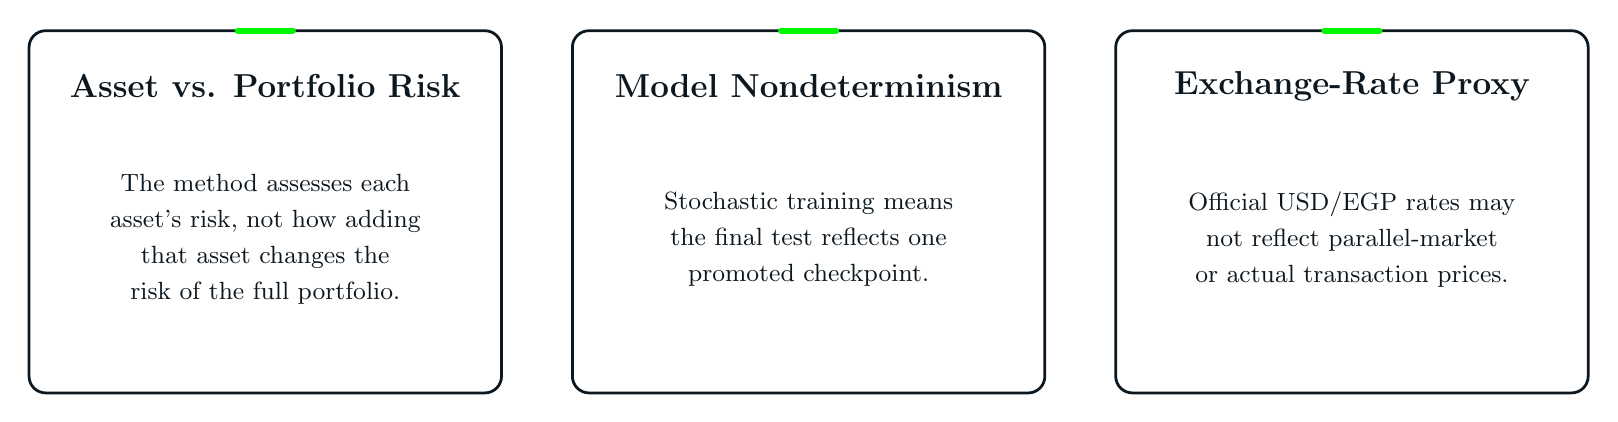
\begin{tikzpicture}

  % --- Card 1: Asset risk versus portfolio risk ---
  \limitationcard{c1}{0}{Asset vs. Portfolio Risk}{%
    The method assesses each asset's risk, not how adding
    that asset changes the risk of the full portfolio.}

  % --- Card 2: Model nondeterminism ---
  \limitationcard{c2}{6.900333}{Model Nondeterminism}{%
    Stochastic training means the final test reflects
    one promoted checkpoint.}

  % --- Card 3: Exchange-rate representation ---
  \limitationcard{c3}{13.800666}{Exchange-Rate Proxy}{%
    Official USD/EGP rates may not reflect parallel-market
    or actual transaction prices.}

\end{tikzpicture}
\end{document}